\textbf{Definition Differentialgleichung:} Eine Gleichung die neben der gesuchten Funktion auch deren Ableitung enthält.\\
\textbf{Gewöhnliche DGL:} Keine partiellen Ableitungen.\\
\textbf{Ordnung:} Höchtse vorkommende Ableitung.\\
\textbf{linear / nicht linear:} nicht linear, wenn die Funktion quadratisch vorkommt.\\
\textbf{homogene DGL:} $y'(x)= h(x)y(x)$\\
\textbf{inhomogene DGL:} $y'(x)= h(x)y(x)+f(x)$\\
\textbf{Ansatz:} Idee zum Lösen einer DGL. Dieser wird in die DGL eingesetzt und anschließend aufgelöst.\\
\textbf{homogene Lösung:} Lösung ohne Störfunktion. ($y_h(x)$) \\
\textbf{partikuläre Lösung:} Lösung mit Störtherm($y_p(x)$) \\
\textbf{allgemeine Lösung:} Lösung der DGL ($y(x)=y_h(x)+y_p(x)$)\\

\textbf{Lösungsverfahren:}
\begin{description}
    \item[Exponentialansatz:] Nur bei \textbf{konstanten Koeffizienten!!}
    \item[Trennen der Variablen:] nur bei \textbf{1. Ordnung.}
    \item[Partikuläre Lösung mit Tabelle:] nur bei \textbf{konstanten Koeffizienten!!}
    \item[Variation der Konstanten:] immer möglich.  
\end{description}

%%
\subsection{Gewöhnliche DGL}
\textbf{implizite Form:} $F(x,y,y',...,y^{(n)})=0$\\
\textbf{explizite Form:} $y^n=f(x,y,y',...,y^{(n-1)})$

%%
\subsubsection{Lösen einer homogenen DGL 1. Ordnung}
$y'(x)=\ga y(x)$
Lösen durch trennen der Variablen oder Exponentialansatz.\\

\textbf{Trennen der Variablen}
\begin{itemize}
    \item $y'$ durch $\frac{dy}{dx}$ ersetzen
    \item alle $y$ und $dy$ sowie $x$ und $dx$ jeweils auf eine Seite bringen.
    \item integrieren
\end{itemize}
$y'(x)=h(x)y(x) \qquad \rightarrow \qquad y(x) = y_0 e ^{\int\limits_{x_0}^{x}h(\tilde{x})d \tilde{x}}$\\

\textbf{Exponentialansatz, nur bei konstanten Koeffizienten!!}\\
$y_0=C\cdot e^{\gl \cdot x}$

\subsubsection{partikuläre Lösung:}

\textbf{mit Tabelle:}
\begin{center}
    \captionsetup{type=figure}
    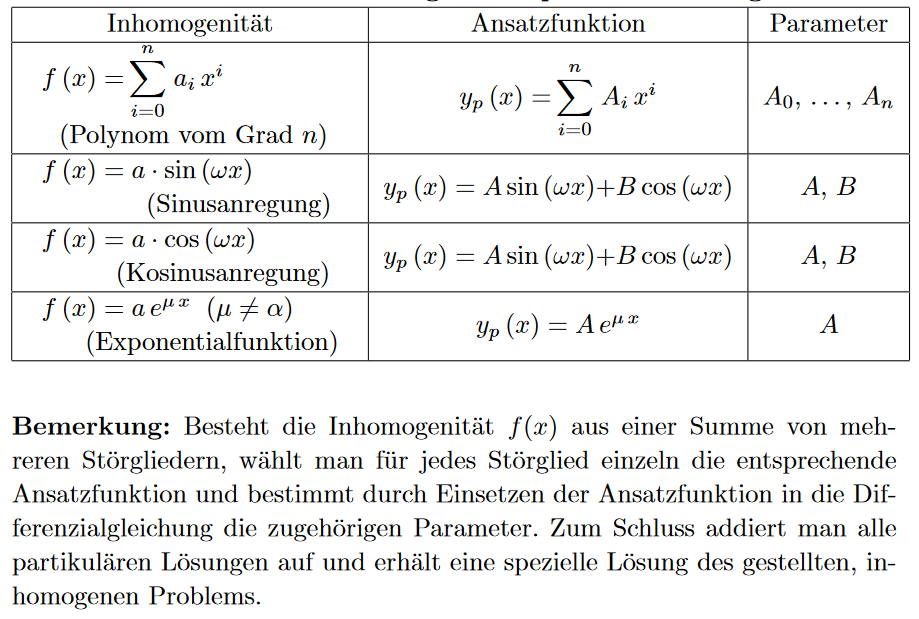
\includegraphics[width=0.9\textwidth]{pictures/Partikuläre_Lösungen_Skript.png}
    \caption{Partikuläre Lösungen}\label{fig:partikuläre_lsg}
\end{center}

Der passende Ansatz wird in die DGL eingesetz und ausgerechnet. Die partikuläre Lösung (bzw. Lösungen bei mehreren Störthermen) werden zur homogenen Lösung addiert und man erhält die Lösung der DGL.\\

\textbf{durch Variation der Konstanten:}
 \[y'(x)=h(x)y(x) + f(x)\]


Berechnen des zugehörigen homogenen Problems $y(x)=C \cdot e ^{\int\limits_{x_0}^{x}h(\tilde{x})d \tilde{x}}$.\\
Die Konstante $C$ wird als variabel $C(x)$ angesehen und der Rest der homogenen Lösung wird $\varphi (x)=e ^{\int\limits_{x_0}^{x}h(\tilde{x})d \tilde{x}}$ geschrieben\\

Es ergibt sich der Ansatz: $\bm{ y(x)=c(x)\cdot \varphi(x)}$, achtung! das ist die \textbf{allgemeine} Lösung\\

Durch Einsetzen von $y(x)$ in die DGL kann man zeigen:

\[c'(x)=\frac{f(x)}{\varphi(x)}\]

somit ist $\bm{c(x) = c_0 + \int\limits_{x_0}^x\frac{f(\tilde{x})}{\varphi(\tilde{x})}d\tilde{x}}$ mit $c_0 = y_0$. 

Eingesetzt in $y(x)$:

\[
    y(x) = \varphi(x) \cdot \left( y_0+\int\limits_{x_0}^x\frac{f(\tilde{x})}{\varphi(\tilde{x})}d\tilde{x}\right)
\]

\subsection{exakte DGL}
Eine DGL 1. Ordnung vom Typ $g(x,y)dx + h(x,y)dy = 0$ ist genau dann \textbf{exaxt}, wenn die Bedingung $\frac{\partial g(x,y)}{\partial y} = \frac{\partial h (x,y)}{\partial x}$ erfüllt ist.\\

Dann ist: $\bm{g(x,y) = \frac{\partial u}{ \partial x}}$ und $\bm{h(x,y) = \frac{\partial u}{ \partial y}}$\\

Durch unbestimmte Integration lässt sich $u(x,y)$ gewinnen, welche in impliziter Form als $u(x,y) = \text{const.} = C$ dargestellt werden kann.\\

$g(x,y)$ muss nach x integriert werden, wobei sich eine Integrationskonstante $K(y)$ ergibt. Um die Integrationskonstante zu bestimmen muss $u(x,y)$ nach $y$ abgeleitet und mit $h(x)$ gleichgesetzt werden. Dann kann $K(y)$ durch integration bestimmt werden. $u(x,y)$ bildet die implizite Lösung und ist konstant ($U(x,y) = \text{const.} = C_2$). Um die explizite Lösung zu erhalten, muss die implizite Lösung $u(x,y) = C_2$ nach $y$ aufgelöst werden.\\

\textbf{Lösen einer exakten DGL:}
\begin{itemize}
    \item $g(x,y)$ nach $x$ integrieren, Integrationskonstante: $K(y)$
    \item $g(x,y)$ nach $y$ ableiten und mit $h(x,y)$ gleichsetzen und damit $K'(y)$ bestimmen
    \item $K(y)$ durch integrieren bestimmen
    \item $u(x,y) = $const. ist die \textbf{implizite Lösung} der DGL
    \item $u(x,y) = C_2$ nach $y$ auflösen --> \textbf{explizite Lösung!}
\end{itemize}

\subsection{DGL 2. Ordnung}

Wenn die DGL linear ist, ist eine Kombination der Lösung durch Addition auch wieder eine Lösung.

Ansatz: $y_0=C\cdot e^{\gl \cdot x}$

\textbf{homogene Lösung} (Skript 2022x12x07 Seite 8)
\begin{itemize}
    \item Ansatz in DGL einsetzen. Dabei die DGL als homogen behandeln.
    \item $C\cdot e^{\gl \cdot x}$ herausheben. Der Rest bildet das charakteristische Polynom.Dieses 0 setzen.
    \item Alle Nullstellen eingesetzt in den Ansatz sind Lösungen der DGL. Die einzelnen Lösungen können linear kombiniert werden, sprich jede Addition von Lösungen ist wieder eine Lösung der DGL. Die \textbf{allgemeine homogene} Lösung ist die Summe der Lösungen, multipliziert mit Konstanten (nur bei linearen DGL). Durch geschicktes Kombinieren von Komplexe Lösungen können reell konstruiert werden.
\end{itemize}

\textbf{partikuläre Lösung}
\begin{itemize}
    \item Partikuläre Lösung von f(x) mit Tabelle bilden.
    \item Homogene und partikuläre Lösung addieren.    
\end{itemize}




\subsection{LDGL, lineare Differenzialgleichungssysteme erster Ordnung mit konstanten Koeffizienten}

\[ \vec{y}´(t)=A\cdot\vec{y}(t) + \vec{f}(t)\]

mit: $I$... Intervall $\vec{f}(t)=\left(
    \begin{array}{r}
        f_1(t)\\
        \vdots\\
        f_n(t)\\
    \end{array} \right) : I \rightarrow \mathbb{R}^n$, $A$... $n\times n$ Matrix.\\
    Ist $f_i(t) = 0$ wird die LDGDL als homogen bezeichnet.






